\documentclass[11pt,a4paper]{article}
\usepackage[margin=1.65cm]{geometry}
\usepackage[T1]{fontenc}
\usepackage[utf8]{inputenc}
\usepackage{booktabs,tabularx,hyperref,xcolor,parskip,enumitem}
\usepackage{tikz}
\usetikzlibrary{arrows.meta,positioning,shapes.geometric,fit,backgrounds,calc}
\usepackage[expansion=false]{microtype}

\definecolor{leafgreen}{HTML}{1B744C}
\definecolor{leafblue}{HTML}{1E5E87}
\definecolor{leafgold}{HTML}{B87512}
\definecolor{leafcoral}{HTML}{B34D45}
\definecolor{leafviolet}{HTML}{6D4C9A}
\definecolor{leafink}{HTML}{22313F}
\definecolor{leafmist}{HTML}{F4F7F6}
\definecolor{leafline}{HTML}{C9D6D0}

\hypersetup{colorlinks=true,linkcolor=leafgreen,urlcolor=leafblue,citecolor=leafviolet}
\setlist[itemize]{nosep,leftmargin=1.35em}
\newcommand{\pathcode}[1]{\texttt{#1}}
\newcommand{\role}[2]{\textcolor{#1}{\textbf{#2}}}

\tikzset{
  flow/.style={-{Stealth[length=2.2mm,width=1.6mm]},thick,draw=leafink!75},
  feedback/.style={-{Stealth[length=2.0mm,width=1.4mm]},thick,dashed,draw=leafviolet},
  box/.style={rounded corners=3pt,draw=leafline,very thick,align=center,minimum height=10mm,inner sep=5pt,font=\small},
  surface/.style={box,fill=leafblue!11,draw=leafblue},
  engine/.style={box,fill=leafgreen!12,draw=leafgreen},
  policy/.style={box,fill=leafgold!14,draw=leafgold},
  provider/.style={box,fill=leafviolet!12,draw=leafviolet},
  evidence/.style={box,fill=leafcoral!10,draw=leafcoral},
  optional/.style={box,fill=black!4,draw=black!35,dashed,text=black!70}
}

\title{\textbf{LeafOS Architecture Atlas}\\[4pt]\large Two-Surface Entry, Guarded Resident Loop, and Durable Evidence}
\author{Synthesized from the reusable root contract, resident architecture, and structure catalog}
\date{2026-07-22}

\begin{document}
\maketitle

\begin{center}
\fcolorbox{leafgreen}{leafmist}{\parbox{0.91\linewidth}{
\textbf{Reading rule.} The colorful paths below are not equal-authority paths.
The PowerShell and Bash surfaces delegate into \pathcode{ProjectLeaf/}; the
current resident taskpack is the execution authority. Models propose bounded
structured content, while CPU-side policy approves, executes, validates, and
checkpoints facts.
}}
\end{center}

\section*{1. The two-surface root delegates to one engine}

\begin{center}
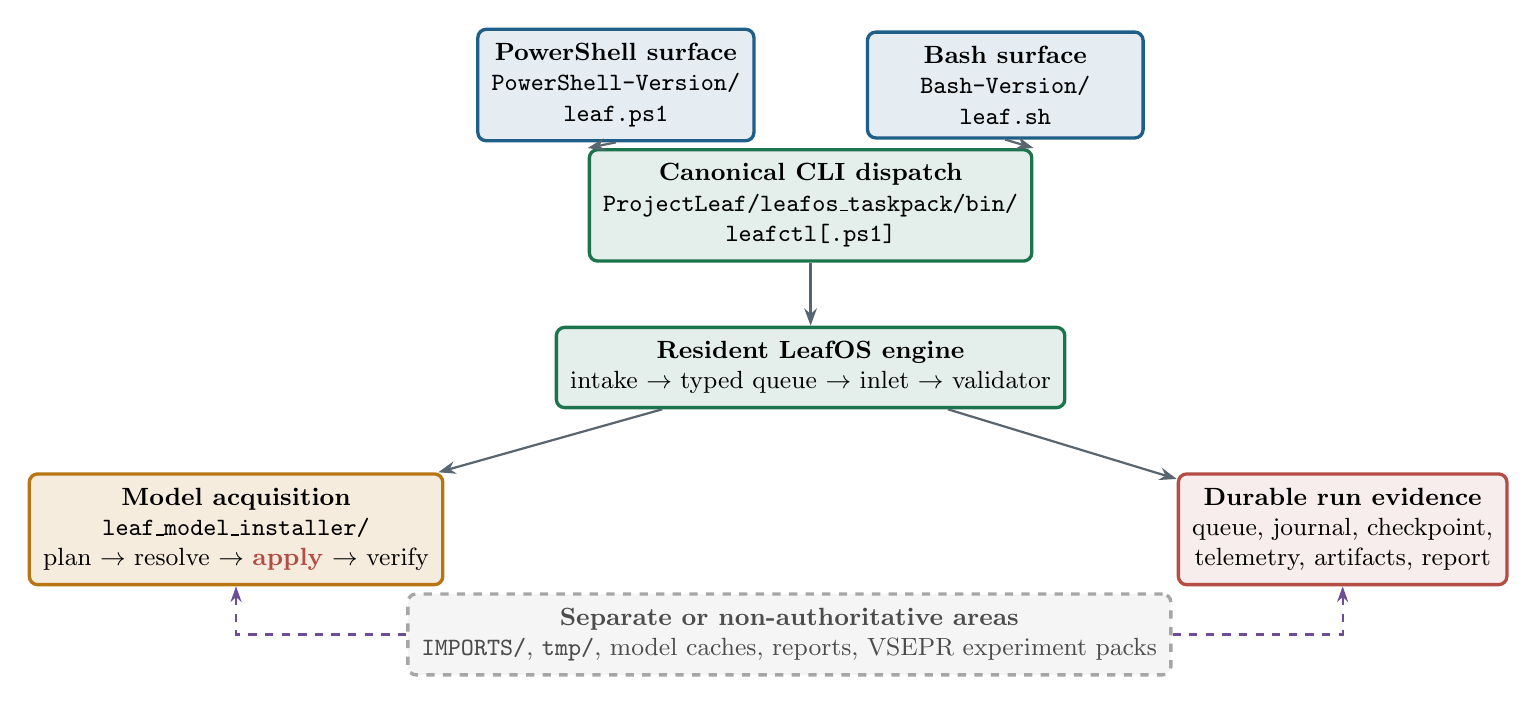
\begin{tikzpicture}[node distance=8mm and 14mm]
  \node[surface,minimum width=35mm] (ps) {\textbf{PowerShell surface}\\\pathcode{PowerShell-Version/}\\\pathcode{leaf.ps1}};
  \node[surface,minimum width=35mm,right=of ps] (bash) {\textbf{Bash surface}\\\pathcode{Bash-Version/}\\\pathcode{leaf.sh}};
  \node[engine,minimum width=50mm,below=of $(ps)!0.5!(bash)$] (cli) {\textbf{Canonical CLI dispatch}\\\pathcode{ProjectLeaf/leafos\_taskpack/bin/}\\\pathcode{leafctl[.ps1]}};
  \node[engine,minimum width=50mm,below=of cli] (loop) {\textbf{Resident LeafOS engine}\\intake \(\rightarrow\) typed queue \(\rightarrow\) inlet \(\rightarrow\) validator};
  \node[policy,minimum width=39mm,below left=of loop] (model) {\textbf{Model acquisition}\\\pathcode{leaf\_model\_installer/}\\plan \(\rightarrow\) resolve \(\rightarrow\) \role{leafcoral}{apply} \(\rightarrow\) verify};
  \node[evidence,minimum width=39mm,below right=of loop] (runs) {\textbf{Durable run evidence}\\queue, journal, checkpoint,\\telemetry, artifacts, report};
  \node[optional,minimum width=55mm,below=of $(model)!0.5!(runs)$] (outside) {\textbf{Separate or non-authoritative areas}\\\pathcode{IMPORTS/}, \pathcode{tmp/}, model caches, reports, VSEPR experiment packs};

  \draw[flow] (ps.south) -- (cli.north west);
  \draw[flow] (bash.south) -- (cli.north east);
  \draw[flow] (cli) -- (loop);
  \draw[flow] (loop) -- (model);
  \draw[flow] (loop) -- (runs);
  \draw[feedback] (outside.west) -| (model.south);
  \draw[feedback] (outside.east) -| (runs.south);
\end{tikzpicture}
\end{center}

\begin{tabularx}{\linewidth}{@{}p{0.24\linewidth}X@{}}
\toprule
\role{leafblue}{Operator surfaces} & Stable entrypoints. They may provide host-specific installation, doctor, chat, and download helpers, but they do not fork taskpack implementation. \\
\role{leafgreen}{Implementation owner} & \pathcode{ProjectLeaf/leafos\_taskpack/} owns task, queue, validation, reporting, provider, UI, and resident-loop behavior. \\
\role{leafgold}{Download boundary} & \pathcode{leaf\_model\_installer/} owns model acquisition. Only explicit \pathcode{apply} may download weights. \\
\role{leafcoral}{Evidence boundary} & Reports, runs, caches, and temporary assets may document execution but never replace source, policy, or validated state. \\
\bottomrule
\end{tabularx}

\section*{2. A local model is a proposal lane, not a control lane}

\begin{center}
\begin{tikzpicture}[node distance=7mm and 9mm]
  \node[surface,minimum width=33mm] (instruction) {\textbf{Instruction}\README/skeleton, project,\\TUI text, JSON task,\\or work order};
  \node[engine,minimum width=35mm,right=of instruction] (intake) {\textbf{Intake}\bounded project facts\\and normalized work};
  \node[provider,minimum width=35mm,right=of intake] (provider) {\textbf{Local provider}\schema-constrained\\proposal only};
  \node[policy,minimum width=38mm,right=of provider] (inlet) {\textbf{CPU inlet}\paths, commands, approvals,\\attempts, ownership};

  \node[policy,minimum width=33mm,below=of intake] (supervisor) {\textbf{Resident supervisor}\resource-aware claim\\and bounded refill};
  \node[engine,minimum width=35mm,below=of provider] (execute) {\textbf{Execute}\tracked, allowlisted\\operations only};
  \node[evidence,minimum width=38mm,below=of inlet] (validate) {\textbf{Validate + commit}\tests, evidence, checkpoint,\\report, bounded repair};

  \draw[flow] (instruction) -- (intake);
  \draw[flow] (intake) -- (provider);
  \draw[flow] (provider) -- (inlet);
  \draw[flow] (inlet) -- (validate);
  \draw[flow] (inlet.south west) -- (execute.north east);
  \draw[flow] (execute) -- (validate);
  \draw[flow] (supervisor) -- (execute);
  \draw[feedback] (validate.west) -| node[pos=0.25,below,font=\scriptsize,text=leafviolet]{bounded repair or next improvement} (supervisor.south);
\end{tikzpicture}
\end{center}

\begin{center}
\begin{tabular}{@{}p{0.24\linewidth}p{0.31\linewidth}p{0.31\linewidth}@{}}
\toprule
Component & May do & Must not do \\
\midrule
\role{leafviolet}{Provider} & Propose a schema-valid plan and bounded content. & Write project files, launch commands, approve itself, or become evidence without validation. \\
\role{leafgold}{Supervisor} & Gate claims from queue, hardware, foreground activity, provider health, and budget. & Bypass the inlet or create unlimited work. \\
\role{leafgreen}{Inlet/executor} & Enforce the accepted work-order boundary and launch tracked work. & Expand authority beyond declared paths, commands, or policy. \\
\role{leafcoral}{Validator} & Run acceptance commands and preserve results. & Convert failure to success or skip required commands. \\
\bottomrule
\end{tabular}
\end{center}

\section*{3. Durable evidence is the restart boundary}

\begin{center}
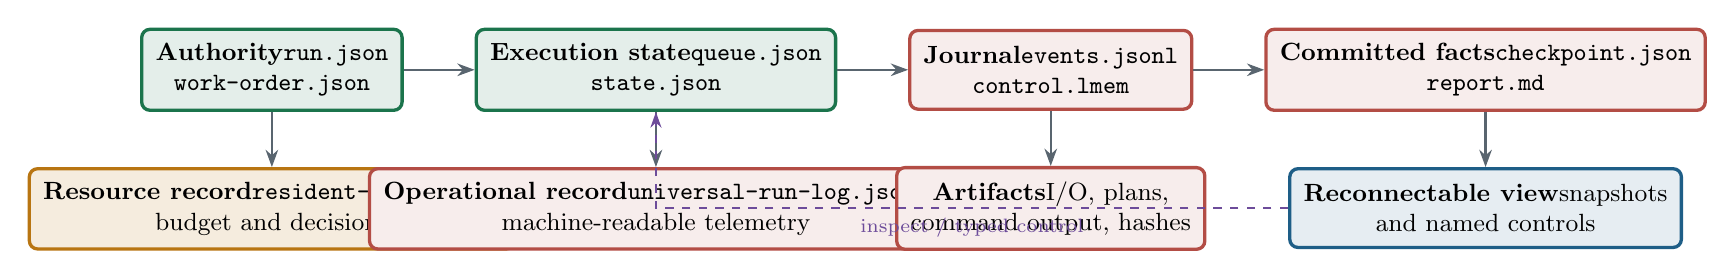
\begin{tikzpicture}[node distance=7mm and 9mm]
  \node[engine,minimum width=31mm] (work) {\textbf{Authority}\pathcode{run.json}\\\pathcode{work-order.json}};
  \node[engine,minimum width=31mm,right=of work] (state) {\textbf{Execution state}\pathcode{queue.json}\\\pathcode{state.json}};
  \node[evidence,minimum width=31mm,right=of state] (journal) {\textbf{Journal}\pathcode{events.jsonl}\\\pathcode{control.lmem}};
  \node[evidence,minimum width=31mm,right=of journal] (checkpoint) {\textbf{Committed facts}\pathcode{checkpoint.json}\\\pathcode{report.md}};

  \node[policy,minimum width=31mm,below=of work] (resident) {\textbf{Resource record}\pathcode{resident-state.json}\\budget and decisions};
  \node[evidence,minimum width=31mm,below=of state] (telemetry) {\textbf{Operational record}\pathcode{universal-run-log.jsonl}\\machine-readable telemetry};
  \node[evidence,minimum width=31mm,below=of journal] (artifacts) {\textbf{Artifacts}\provider I/O, plans,\\command output, hashes};
  \node[surface,minimum width=31mm,below=of checkpoint] (ui) {\textbf{Reconnectable view}\normalized snapshots\\and named controls};

  \draw[flow] (work) -- (state);
  \draw[flow] (state) -- (journal);
  \draw[flow] (journal) -- (checkpoint);
  \draw[flow] (work) -- (resident);
  \draw[flow] (state) -- (telemetry);
  \draw[flow] (journal) -- (artifacts);
  \draw[flow] (checkpoint) -- (ui);
  \draw[feedback] (ui.west) -| node[pos=0.25,below,font=\scriptsize,text=leafviolet]{inspect / typed control} (state.south);
\end{tikzpicture}
\end{center}

\begin{center}
\fcolorbox{leafcoral}{leafcoral!7}{\parbox{0.90\linewidth}{
\textbf{Fact hierarchy.} A model plan or reflection is a record, not evidence.
Validation produces checkable evidence. A checkpoint commit is the only source
of authoritative resume position, task state, and \pathcode{next\_action}.
Short-lived lease files describe ownership while a process exists; they are not
durable truth after it exits.
}}
\end{center}

\section*{4. Directory legend: what to read, run, or leave alone}

\begin{tabularx}{\linewidth}{@{}p{0.27\linewidth}p{0.19\linewidth}X@{}}
\toprule
Path / material & Visual role & Practical interpretation \\
\midrule
\pathcode{markdowns/ROOT\_CONTRACT.md} & \role{leafblue}{Blue: entry} & Reusable root layout, shell ownership, and safe defaults. \\
\pathcode{ProjectLeaf/leafos\_taskpack/} & \role{leafgreen}{Green: engine} & Current resident implementation, schemas, CLI, tests, and operational guides. \\
\pathcode{ProjectLeaf/leaf\_model\_installer/} & \role{leafgold}{Gold: guarded input} & Canonical model catalog and explicit download workflow. \\
\pathcode{IMPORTS/} & \role{leafviolet}{Violet: reference} & Imported compatibility/source snapshot. Read for history or a named subsystem; do not let it override current resident documents. \\
\pathcode{runs/}, \pathcode{reports/}, \pathcode{logs/} & \role{leafcoral}{Coral: evidence} & Generated evidence. Inspect and preserve; do not treat as source authority. \\
\pathcode{tmp/}, \pathcode{.venv/}, \pathcode{.vs/}, model caches & \role{leafcoral}{Coral: disposable} & Tooling, IDE state, downloaded binaries, or local models. Rebuild/reacquire rather than modifying as product source. \\
\pathcode{VSEPR-Day98-LeafOS-Run1/} & \role{leafviolet}{Violet: experiment} & Isolated scientific loop contract; promotion requires its own verified gates and explicit apply authorization. \\
\bottomrule
\end{tabularx}

\section*{5. Recommended architecture reading sequence}

\begin{enumerate}[leftmargin=1.55em]
  \item Read \pathcode{ROOT\_CONTRACT.md} for the shell-surface and ownership split.
  \item Read \pathcode{ProjectLeaf/leafos\_taskpack/README.md} for resident behavior and first commands.
  \item Read \pathcode{docs/DOCUMENTATION\_MAP.md} to distinguish current contracts from optional or historical documentation.
  \item Read \pathcode{docs/ARCHITECTURE.md} beside the three diagrams in this atlas.
  \item Read \pathcode{docs/AGENTIC\_CLI.md} for instruction normalization and the guarded lifecycle.
  \item Read \pathcode{docs/MEMORY\_MODEL.md} for record, evidence, and committed-fact rules.
\end{enumerate}

\section*{6. Behavior panels}

\subsection*{6.1 Project onboarding and \pathcode{live} \hfill \role{leafgreen}{IMPLEMENTED}}

\begin{center}
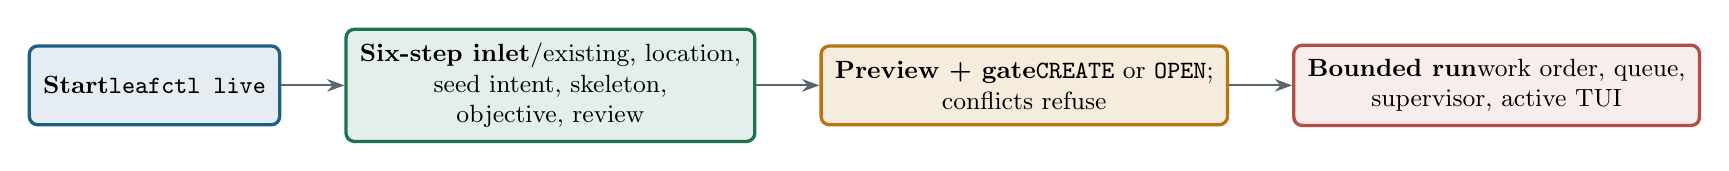
\begin{tikzpicture}[node distance=7mm and 8mm]
  \node[surface,minimum width=30mm] (start) {\textbf{Start}\pathcode{leafctl live}};
  \node[engine,minimum width=34mm,right=of start] (form) {\textbf{Six-step inlet}\new/existing, location,\\seed intent, skeleton,\\objective, review};
  \node[policy,minimum width=34mm,right=of form] (gate) {\textbf{Preview + gate}\type \pathcode{CREATE} or \pathcode{OPEN};\\conflicts refuse};
  \node[evidence,minimum width=34mm,right=of gate] (run) {\textbf{Bounded run}\intake work order, queue,\\supervisor, active TUI};
  \draw[flow] (start)--(form); \draw[flow] (form)--(gate); \draw[flow] (gate)--(run);
\end{tikzpicture}
\end{center}

Existing projects are read-only during intake and receive no LeafOS control
files. A new project creates exactly \pathcode{README.md}, \pathcode{skeleton.md},
and \pathcode{leafos.project.json}. The requested KV-cache preference is a
priority task recorded as \pathcode{applied: false}; it becomes applied only
after a reversible project-owned launch change, validation, and throughput/VRAM
evidence. It never restarts a shared provider directly.

\subsection*{6.2 Resource governor and lifecycle controls \hfill \role{leafgreen}{IMPLEMENTED}}

\begin{center}
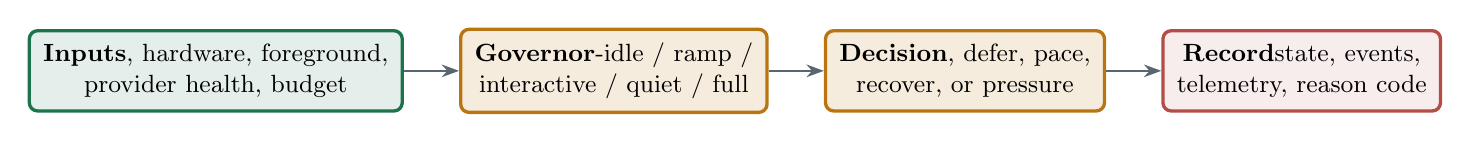
\begin{tikzpicture}[node distance=6mm and 7mm]
  \node[engine,minimum width=31mm] (facts) {\textbf{Inputs}\queue, hardware, foreground,\\provider health, budget};
  \node[policy,minimum width=34mm,right=of facts] (governor) {\textbf{Governor}\auto-idle / ramp /\\interactive / quiet / full};
  \node[policy,minimum width=31mm,right=of governor] (decision) {\textbf{Decision}\claim, defer, pace,\\recover, or pressure};
  \node[evidence,minimum width=31mm,right=of decision] (record) {\textbf{Record}\resident state, events,\\telemetry, reason code};
  \draw[flow] (facts)--(governor); \draw[flow] (governor)--(decision); \draw[flow] (decision)--(record);
\end{tikzpicture}
\end{center}

CPU/GPU values are useful-work targets, not load quotas. Missing counters stay
unknown; the stack does not create duplicate inference or meaningless CPU work
to inflate utilization. \pathcode{pause} stops new claims at a safe boundary,
\pathcode{drain} finishes accepted work while rejecting admission, \pathcode{stop}
uses confirmed cancellation, and \pathcode{resume} ensures one supervisor.

\subsection*{6.3 Provider routing and degraded recovery \hfill \role{leafgold}{EVIDENCE-GATED}}

\begin{center}
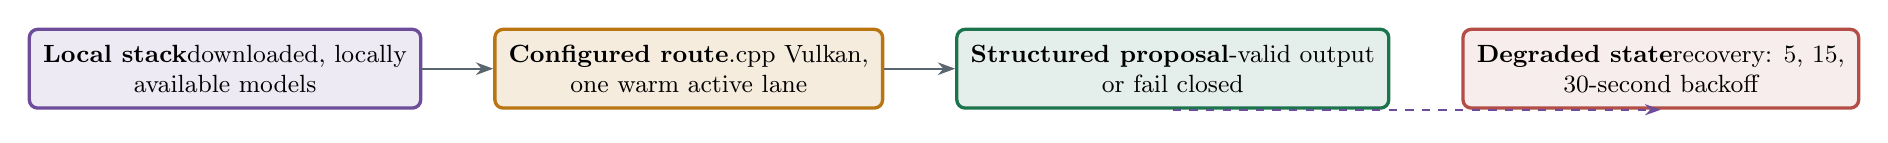
\begin{tikzpicture}[node distance=7mm and 9mm]
  \node[provider,minimum width=35mm] (stack) {\textbf{Local stack}\all downloaded, locally\\available models};
  \node[policy,minimum width=35mm,right=of stack] (route) {\textbf{Configured route}\llama.cpp Vulkan,\\one warm active lane};
  \node[engine,minimum width=35mm,right=of route] (proposal) {\textbf{Structured proposal}\schema-valid output\\or fail closed};
  \node[evidence,minimum width=35mm,right=of proposal] (degraded) {\textbf{Degraded state}\tracked recovery: 5, 15,\\30-second backoff};
  \draw[flow] (stack)--(route); \draw[flow] (route)--(proposal); \draw[feedback] (proposal.south) |- (degraded.south);
\end{tikzpicture}
\end{center}

The current route remains the Q3 coding path until a named candidate passes the
4-, 8-, and 64-minute qualification portfolio and receives operator approval.
A provider failure is visible and never becomes mock output or CPU-invented
model text. Medium-MoE selection is a research and qualification contract, not
a claim that an unresolved candidate is active.

\subsection*{6.4 Memory, checkpoint, and resume \hfill \role{leafblue}{FOUNDATION IMPLEMENTED; PIPELINE IN PROGRESS}}

\begin{center}
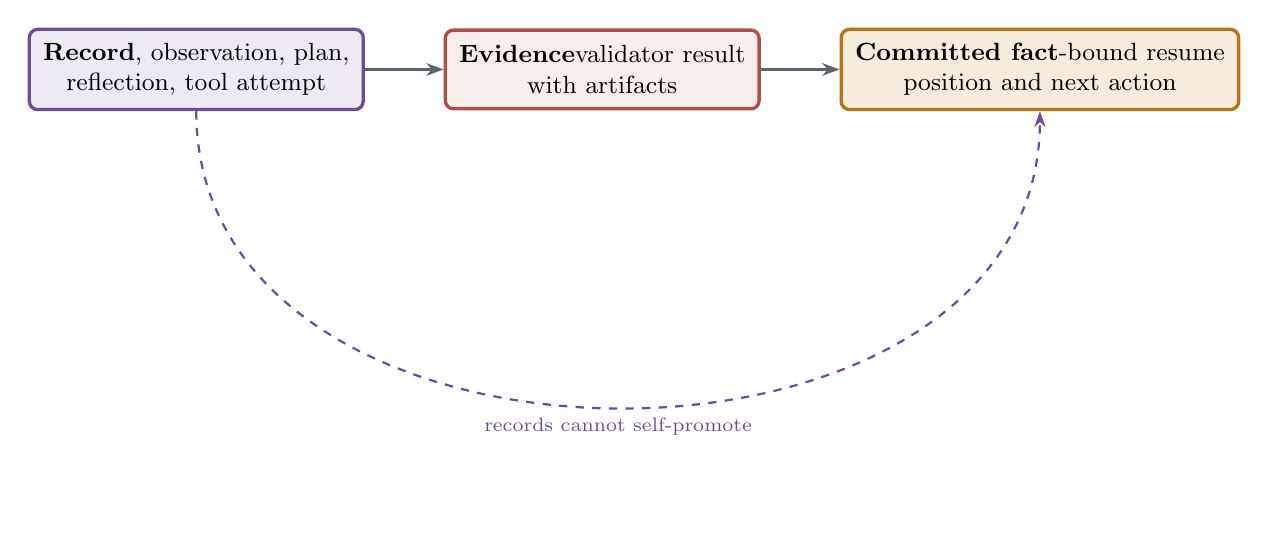
\begin{tikzpicture}[node distance=7mm and 10mm]
  \node[provider,minimum width=35mm] (record) {\textbf{Record}\request, observation, plan,\\reflection, tool attempt};
  \node[evidence,minimum width=35mm,right=of record] (evidence) {\textbf{Evidence}\checkable validator result\\with artifacts};
  \node[policy,minimum width=35mm,right=of evidence] (fact) {\textbf{Committed fact}\checkpoint-bound resume\\position and next action};
  \draw[flow] (record)--(evidence); \draw[flow] (evidence)--(fact);
  \draw[feedback] (record.south) to[out=-90,in=-90,looseness=1.2] node[below,font=\scriptsize,text=leafviolet]{records cannot self-promote} (fact.south);
\end{tikzpicture}
\end{center}

Native LMEM supplies sealed, sequence-checked journal records and verified
replay; \pathcode{events.jsonl} supports reconnectable presentation;
\pathcode{checkpoint.json} holds validated recovery facts. The SQLite/FTS
projection is disposable cache state. Reflection/context-pack features remain
bounded, non-authoritative, and subject to the committed-fact boundary.

\subsection*{6.5 TUI, telemetry, and reconnectable monitoring \hfill \role{leafgreen}{LARGELY COMPLETE}}

\begin{center}
\begin{tikzpicture}[node distance=7mm and 9mm]
  \node[evidence,minimum width=34mm] (snapshot) {\textbf{Normalized snapshot}\tasks, milestones, hardware,\\ledger, results, cursor};
  \node[surface,minimum width=34mm,right=of snapshot] (renderers) {\textbf{Two renderers}\native \pathcode{ncursesw} or\\Python ANSI fallback};
  \node[policy,minimum width=34mm,right=of renderers] (bridge) {\textbf{Typed controls}\loopback token, named\\actions, validated task IDs};
  \node[engine,minimum width=34mm,right=of bridge] (inlet) {\textbf{Loop inlet}\the only queue and\\execution authority};
  \draw[flow] (snapshot)--(renderers); \draw[flow] (renderers)--(bridge); \draw[flow] (bridge)--(inlet);
\end{tikzpicture}
\end{center}

The seven pages show overview, tasks, hardware, queue, provider progress,
ledger, and results. The independent hardware sampler presents live CPU, RAM,
GPU, VRAM, temperature, and power with sample age without rewriting the durable
ledger. Both renderers support guided onboarding and authenticated typed
controls; neither schedules work, edits queues, or executes arbitrary shell
text. \pathcode{q} closes only the view, while \pathcode{--json} and JSONL
monitoring support noninteractive observation.

\section*{Operational doctrine}

\begin{center}
\textcolor{leafgreen}{\textbf{Inspect}} \(\rightarrow\)
\textcolor{leafviolet}{\textbf{propose}} \(\rightarrow\)
\textcolor{leafgold}{\textbf{approve}} \(\rightarrow\)
\textcolor{leafblue}{\textbf{execute}} \(\rightarrow\)
\textcolor{leafcoral}{\textbf{validate and checkpoint}}
\end{center}

The central safety property is deliberate asymmetry: the model may suggest,
but it cannot make an unreviewed suggestion true, executable, or durable.

\end{document}
